\section{影像分类实验}




\subsection{分类流程}
\begin{frame}{当前章节}
    \tableofcontents[currentsection, currentsubsection]
\end{frame}

\begin{frame}{分类流程}
    \begin{columns}
        \column{0.5\textwidth}
        \begin{itemize}
            \item 分类方法: 无监督Kmeans聚类; 监督: 深度学习的方法
            \item 分类结果
            \item 对分类结果进行Label可视化
            \item 与真值对比进行分类精度的评定 
        \end{itemize}

        \column{0.5\textwidth}
        \begin{figure}
            \centering
            % Requires \usepackage{graphicx}
            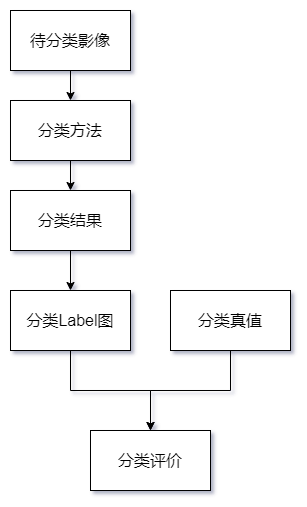
\includegraphics[height=5cm]{pic/pic0202.png}
            \caption{分类流程}
            \label{fig:0101}
        \end{figure}
    \end{columns}
\end{frame}

\subsection{分类实验结果}
\begin{frame}{当前章节}
    \tableofcontents[currentsection, currentsubsection]
\end{frame}

\begin{frame}{分类实验结果}
    \begin{figure}[!htbp]
        \centering
        \subfloat[origin]{\label{fig:0203a}
        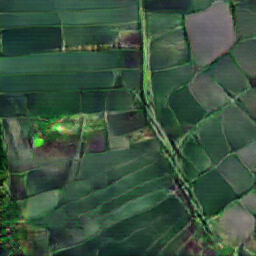
\includegraphics[height=4cm]{pic/pic0203origin.png}}
        \quad
        \subfloat[predict]{\label{fig:0203b}
        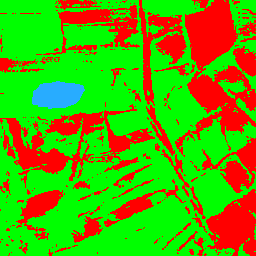
\includegraphics[height=4cm]{pic/pic0203predict.png}}
        \caption{Kmeans聚类结果}
        \label{fig:0203}
    \end{figure}
\end{frame}

\begin{frame}{分类实验结果}
    \begin{figure}[!htbp]
        \centering
        \subfloat[predict]{\label{fig:0203a}
        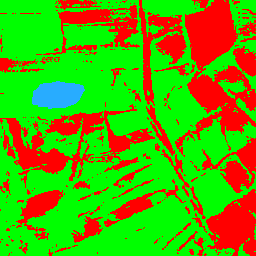
\includegraphics[height=4cm]{pic/pic0203predict.png}}
        \quad
        \subfloat[groudtruth]{\label{fig:0203b}
        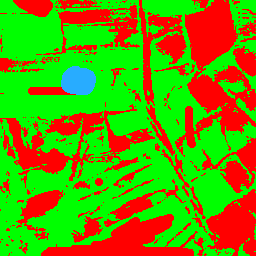
\includegraphics[height=4cm]{pic/pic0203truth.png}}
        \caption{预测与真值}
        \label{fig:0203}
    \end{figure}
\end{frame}

\begin{frame}{分类实验结果}
    \begin{table}[h]
        \centering
        \begin{tabular}{ m{2cm} | m{2cm} | m{2cm} | m{2cm} | }
            \hline
             & class1 & class2 & class3 \\ \hline
            class1 & 21814 & 0 & 1 \\ \hline       
            class2 & 3576  & 38428 & 596 \\ \hline
            class3 & 252  &  646 &  223 \\ \hline            
        \end{tabular}
        \caption{混淆矩阵}
    \end{table}

    \begin{table}[h]
        \centering
        \begin{tabular}{ m{2cm} | m{2cm} | m{2cm} | m{2cm} | }
            \hline
             & class1 & class2 & class3 \\ \hline
            精度 & 85.07\% & 98.34\% & 27.19\% \\ \hline       
            召回率 & 99.99\% & 90.20\% & 19.89\% \\ \hline
        \end{tabular}
        \caption{混淆矩阵}
    \end{table}
\end{frame}

\subsection{数据准备}
\begin{frame}{当前章节}
    \tableofcontents[currentsection, currentsubsection]
\end{frame}

\begin{frame}{数据准备}
    遥感影像语义分割数据集:
    \begin{itemize}
        \item Gaofen Image Dataset(GID)
        \item DeepGlobe Land Cover Classification Challenge
        \item SEN12MS
    \end{itemize}
\end{frame}

\begin{frame}{GID数据}
    GID用高分2号数据做成的大范围土地利用覆盖数据集. 
    \begin{figure}[!htbp]
        \centering
        \subfloat[input]{\label{fig:0201a}
        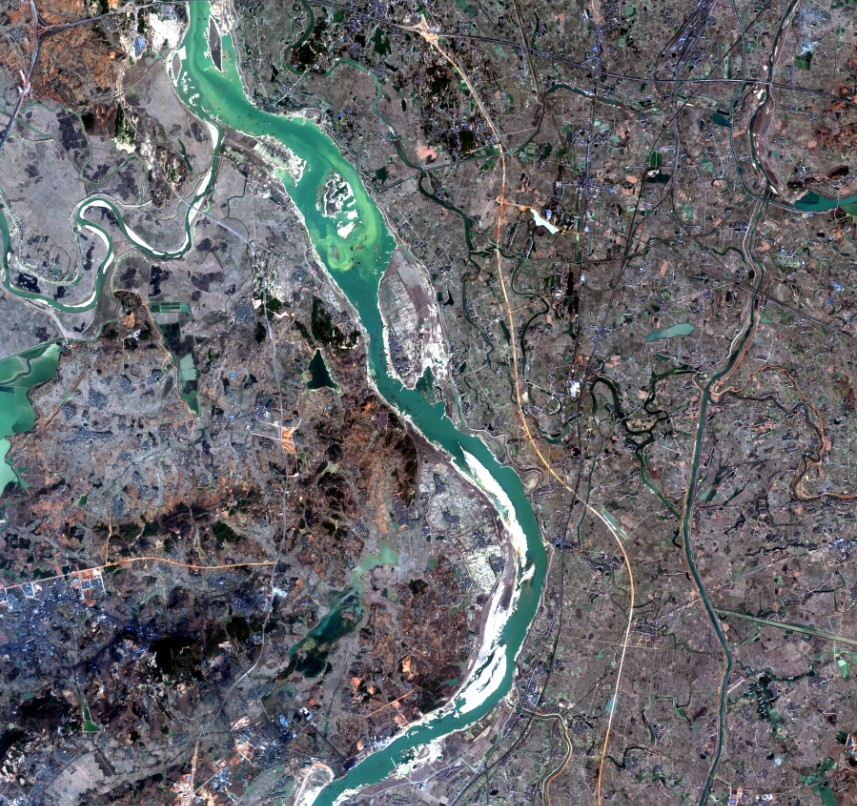
\includegraphics[height=4cm]{pic/pic0201a.jpg}}
        \quad
        \subfloat[output]{\label{fig:0201b}
        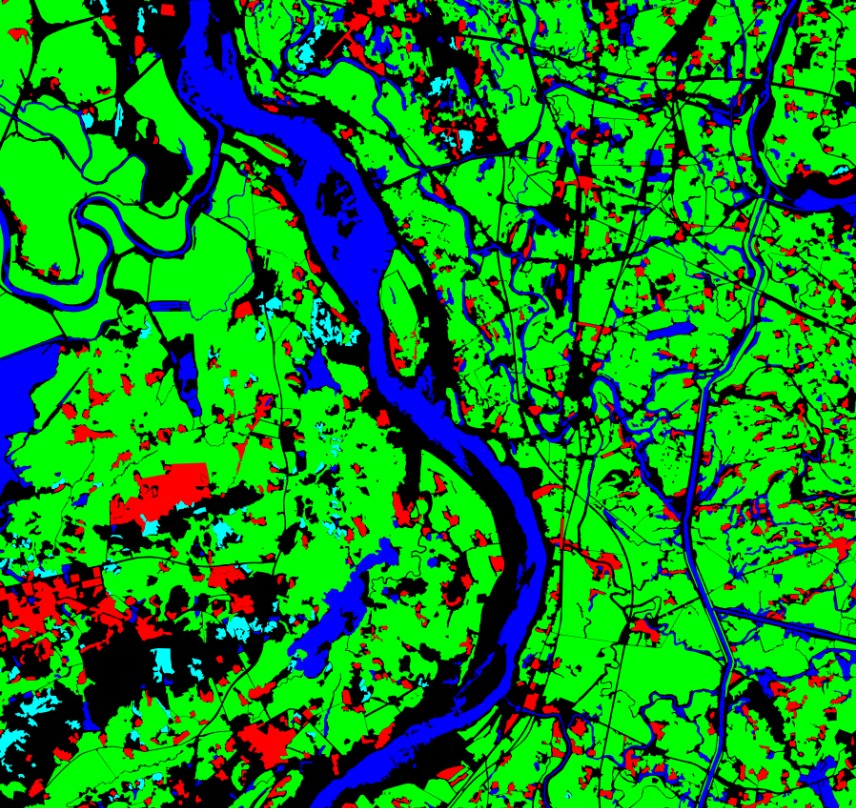
\includegraphics[height=4cm]{pic/pic0201b.jpg}}
        \caption{GID 数据}
        \label{fig:0201}
    \end{figure}
\end{frame}

\subsection{工作计划}
\begin{frame}{当前章节}
    \tableofcontents[currentsection, currentsubsection]
\end{frame}

\begin{frame}{工作计划}
    在matlab中实现:
    \begin{itemize}
        \item 根据GID数据集, 给数据加标签制作数据集
        \item 使用matlab进行多个模型的训练
        \item 对整体图像翻译进行分类, 并进行结果评定
    \end{itemize}
\end{frame}

